\chapter{Aporte práctico}

En el capítulo 3 se presentaron algunas técnicas y herramientas que sirven para el aprendizaje colaborativo; No obstante, para objetivos de esta tesis, se requiere una herramienta que integre ciertas características de las que ya poseen las mencionadas en el capítulo anterior. Ver Tabla \ref{tab:herramientasAC}.\\

El sistema que se pretende desarrollar estará basado en el proceso para la elaboración de sesiones de clase usando la técnica de Jigsaw en la cual, tanto los grupos expertos y grupos jigsaw serán generados aleatoriamente por el sistema, garantizando así una mayor interacción entre los estudiantes, especialmente entre aquellos que se conocen por primera vez. Ver Tabla \ref{tab:tecnicasAC}.\\

El sistema a desarrollar también tendrá la particularidad de que permitirá a los estudiantes trabajar de forma colaborativa en la elaboración de archivos de código fuente, los cuales serán producto de las respuestas que dichos estudiantes darán a los problemas que les plantee el profesor durante la sesión de clase jigsaw. Por ende, para lograr este objetivo y tener dicha funcionalidad en el sistema, se usará los frameworks y APIs descritas en el capítulo anterior. Ver tabla \ref{tab:frameworks}.\\

Finalmente, para el desarrollo del sistema web, al cual de ahora en adelante llamaremos \textbf{Sistema Jigsaw Coding}, se va a considerar como proceso de desarrollo a las mejores prácticas de RUP para garantizar un producto software de calidad.

\section{Metodología de desarrollo}
Como ya se mencionó anteriormente, el Sistema Jigsaw Coding será elaborado usando las mejores prácticas de RUP, el mismo que a continuación se describe brevemente:\\

EL Proceso Unificado Rational(RUP) es un proceso de ingeniería de software que provee un enfoque para la asignación de tareas y responsabilidades durante el desarrollo de un software. Este tiene como objetivo asegurar la producción de un producto software de alta calidad que satisfaga los requerimientos de los usuarios finales dentro de un tiempo y presupuesto establecido \cite{rup_ibm_2014}. RUP, divide el proceso de desarrollo en fases y agrupa las diversas tareas y actividades en disciplinas, permitiendo organizar eficientemente cada uno de los artefactos que serán producto del desarrollo del sistema. Ver figura \ref{fig:rup}\\

\begin{figure}[!h]
  \centering
  % Requires \usepackage{graphicx}
  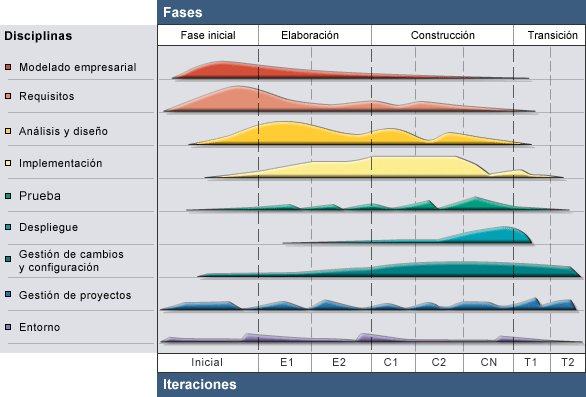
\includegraphics[scale=0.7]{figuras/rup.jpg}\\
  \caption[RUP]{Proceso de desarrollo de software - RUP \protect\cite{rup_small}}\label{fig:rup}
\end{figure}

Así mismo, RUP también es una guía para usar de manera efectiva el Lenguaje Unificado de Modelado (UML) que no es más que un lenguaje estándar que permite comunicar claramente los requerimientos, arquitecturas y diseños \cite{rup_ibm_2014}.\\

Para el desarrollo del Sistema Jigsaw Coding, se establecerán iteraciones semanales en las cuales se irá desarrollando cada una de las fases en las que RUP divide el ciclo de desarrollo de software: Inicio, Elaboración, Construcción y Transición. Los artefactos que serán entregados durante el proceso de desarrollo del sistema propuesto en esta tesis se mencionan en la Tabla \ref{tab:artefactos_rup}. Además, dichos artefactos se encuentran agrupados según la disciplina a la que pertenecen.

\begin{longtable}{|L{6cm}|L{7cm}|}
\caption{Artefactos del proceso de desarrollo del Sistema Jigsaw Coding}
\label{tab:artefactos_rup}\\
    \hline
    DISCIPLINA RUP & ARTEFACTO \\
    \hline
    \multirow{2}{*}{Requisitos} & $\bullet$ Modelo de caso de uso\\
    \hhline{~~} & $\bullet$ Especificaciones de casos de uso\\
    \hhline{~~} & $\bullet$ Especificaciones suplementarias\\
    \hline
    \multirow{5}{*}{Análisis y diseño} & $\bullet$ Diagrama de clases\\
    \hhline{~~} & $\bullet$ Modelo de datos\\
    \hhline{~~} & $\bullet$ Prototipo de interfaz de usuario\\
    \hhline{~~} & $\bullet$ Documento de arquitectura de software\\
    \hline
    \multirow{2}{*}{Implementación} & $\bullet$ Código fuente\\
    \hhline{~~} & $\bullet$ Sistema web desplegado\\
    \hline
    \multirow{2}{*}{Prueba} & $\bullet$ Casos de prueba\\
    \hhline{~~} & $\bullet$ Resultados de prueba\\
    \hline
\end{longtable}

\clearpage
%Para el desarrollo del sistema web, se seguirá el siguiente cronograma, el mismo que se está orientado a seguir las actividades y tareas que plantea RUP. Se indica también las fechas en las cuales se estará aplicando el sistema al caso de estudio.
%
%\begin{figure}[!h]
%  \centering
%  % Requires \usepackage{graphicx}
%  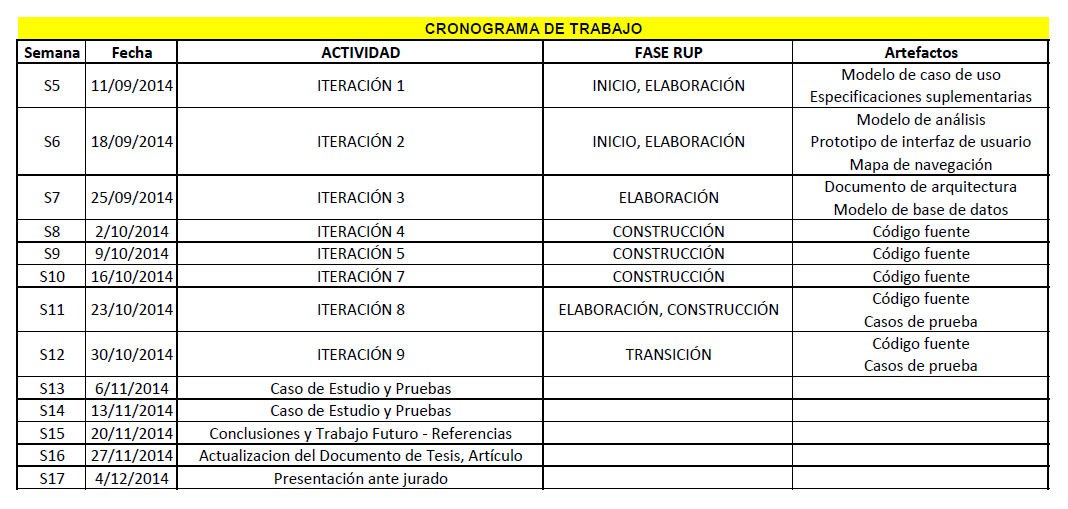
\includegraphics[scale=0.5]{figuras/cronograma.png}\\
%  \caption[CRONOGRAMA]{Cronograma de trabajo}\label{fig:cronograma}
%\end{figure}

%\begin{longtable}{|L{2.5cm}|L{2cm}|L{5cm}|L{5cm}|}
%\caption{CRONOGRAMA}
%\label{tab:cronograma}\\
%    \hline
%    ITERACIÓN & FECHA & FASE RUP & ARTEFACTO \\
%    \hline
%    1 &	11-09-2014	&	INICIO, ELABORACIÓN	& Modelo de caso de uso, Especificaciones suplementarias\\
%
%    \hline
%\end{longtable}

\section{Desarrollo del Sistema Jigsaw Coding}

\section{Uso del Sistema Jigsaw Coding} 
El Sistema Jigsaw Coding es un aplicativo web que permite crear sesiones de clase basadas en la técnica de aprendizaje colaborativo de rompecabezas o también llamada técnica jigsaw. Estas sesiones de clase están orientadas a la resolución de ejercicios y problemas relacionados con temas de algorítmica y programación en lenguajes Java, C++ y Python.\\

El sistema posee dos perfiles de usuario: Docente y Alumno. El primero permite al usuario crear ejercicios y problemas de algoritmos y programación. Dentro del perfil docente, el usuario tiene la capacidad para crear a los usuarios alumnos que participarán en la sesión de clase jigsaw para luego asignarlos a las sesiones jigsaw para que el sistema genere los grupos expertos y grupos jigsaw. Posteriormente a ello, el usuario con perfil docente podrá asignar a cada grupo experto un problema o ejercicio a resolver, y luego asignar la fecha y duración para cada fase de la dinámica jigsaw (Reunión de Expertos, Reunión Jigsaw y Evaluación). Para la fase de evaluación, el sistema permite al usuario crear diversos examenes con problemas y ejercicios a los cuales se les asigna un puntaje; luego, cada examen se asigna a una determinada sesión jigsaw. Finalmente, el usuario docente podrá calificar la solución que cada uno de los participantes de la sesión jigsaw elabore para un determinado examen.\\

En el perfil Alumno, el usuario puede participar de las reuniones de expertos y reunions jigsaw, en las cuales se deberá resolver los problemas asignados a cada grupo experto o jigsaw. Esta soluciones serán construidas de forma colaborativa entre todos los miembros de cada grupo. El sistema brinda al usuario un chat para poder comunicarse con los demás integrantes de su grupo experto o jigsaw. Es importante resaltar también, que durante la resolución de cada problema el usuario puede ir ejecutando el código fuente y ver los resultados de dicha ejecución. Cuando el usuario se encuentre en la fase de evaluación, éste podrá resolver su examen de forma individual y dentro del tiempo establecido por el docente.\\

\subsection{Login} 
Para acceder al Sistema Jigsaw Coding, el usuario debe estar su \textbf{email} y su \textbf{password} en el formulario que se muestra en la figura \ref{fig:sjc_login}.

\begin{figure}[h!]
	\centering
	\caption[SJC Login]{Sistema Jigsaw Coding - Login}
	\label{fig:sjc_login}
	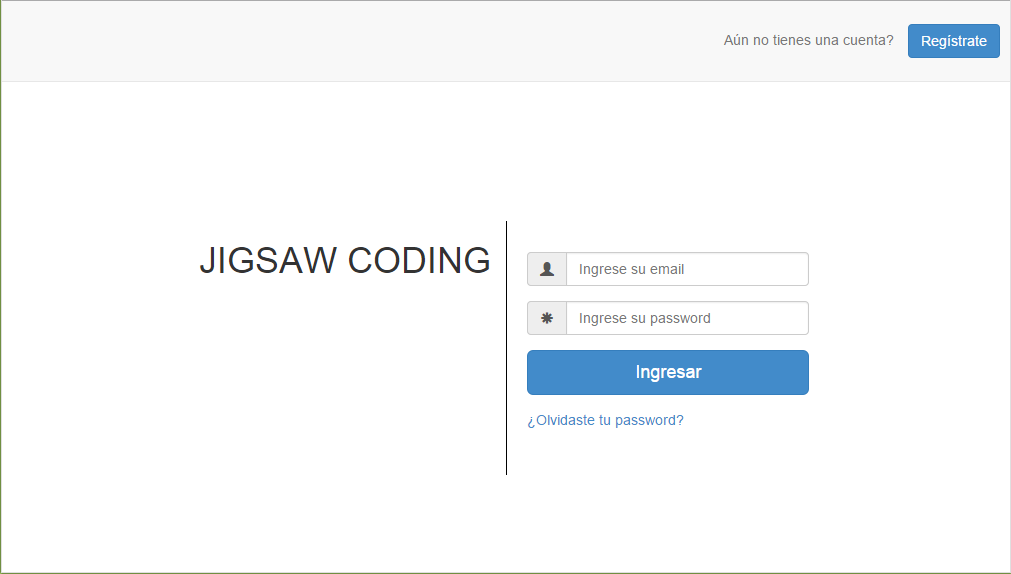
\includegraphics[scale=0.4]{figuras/usodelsistema/login}	
\end{figure}

Si el usuario no está registrado en el sistema, debe ingresar a la opción \textbf{Regístrate} y completar los datos solicitados por el sistema. Ver figura \ref{fig:login_registrate}. Luego de este paso, el usuario tendrá acceso al sistema a través de un perfil Docente.\\

\begin{figure}[h!]
	\centering
	\caption[SJC Registrate]{Sistema Jigsaw Coding - Regístrate}
	\label{fig:login_registrate}
	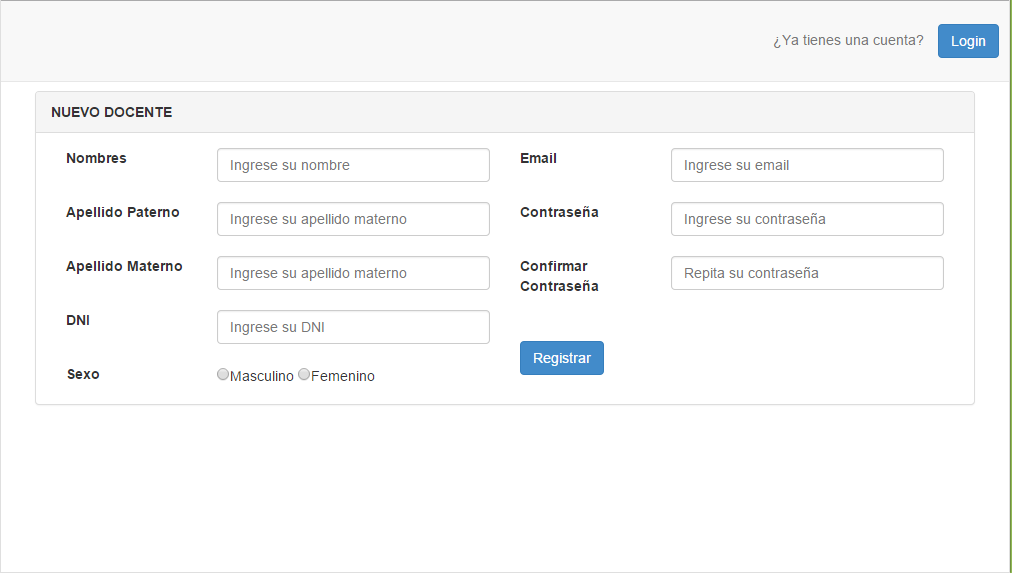
\includegraphics[scale=0.5]{figuras/usodelsistema/login_registrate}	
\end{figure}

Si el acceso al sistema se dió exitosamente, entonces el usuario podrá visualizar la página de inicio con todas las opciones permitidas para el perfil docente. Ver figura \ref{fig:inicio}.

\begin{figure}[h!]
\centering
\caption[SJC Inicio]{Sistema Jigsaw Coding - Bienvenido}
\label{fig:inicio}
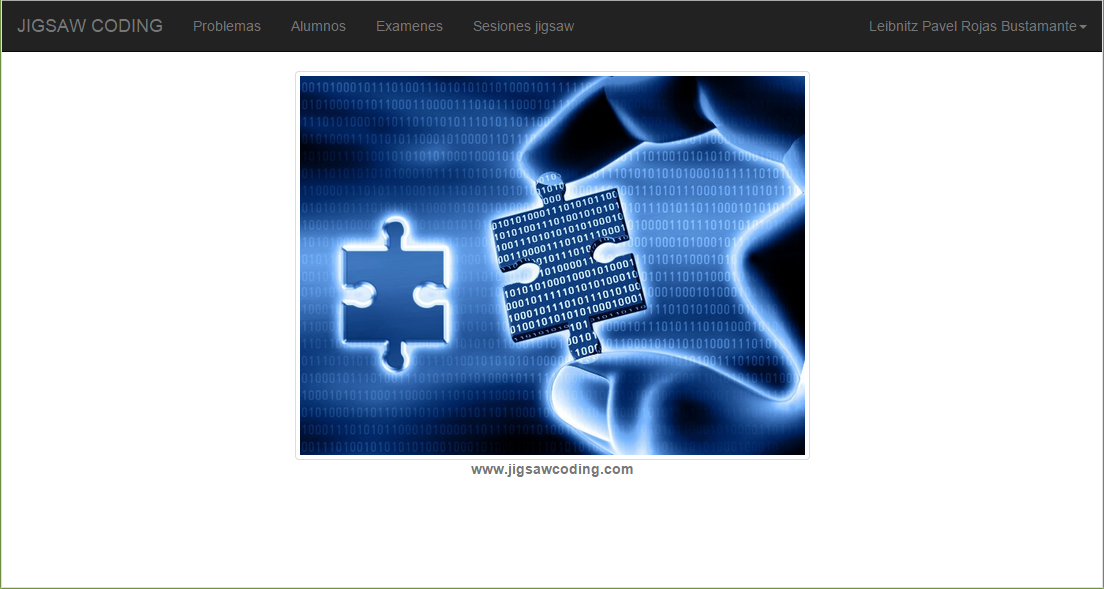
\includegraphics[scale=0.5]{figuras/usodelsistema/docente/inicio}
\end{figure}
\clearpage
\section*{Perfil Docente}

\subsection{Problemas}
Al acceder al módulo problemas, el usuario visualizará el listado de problemas que ha creado hasta el momento y en dicho listado, se mostrará el título y enunciado de cada problema. Además se podrá filtrar los problemas según el título o enunciado. Ver figura \ref{fig:problemas_inicio}.

\begin{figure}[h!]
\centering
\caption[SJC Problemas]{Sistema Jigsaw Coding - Inicio del módulo Problemas}
\label{fig:problemas_inicio}
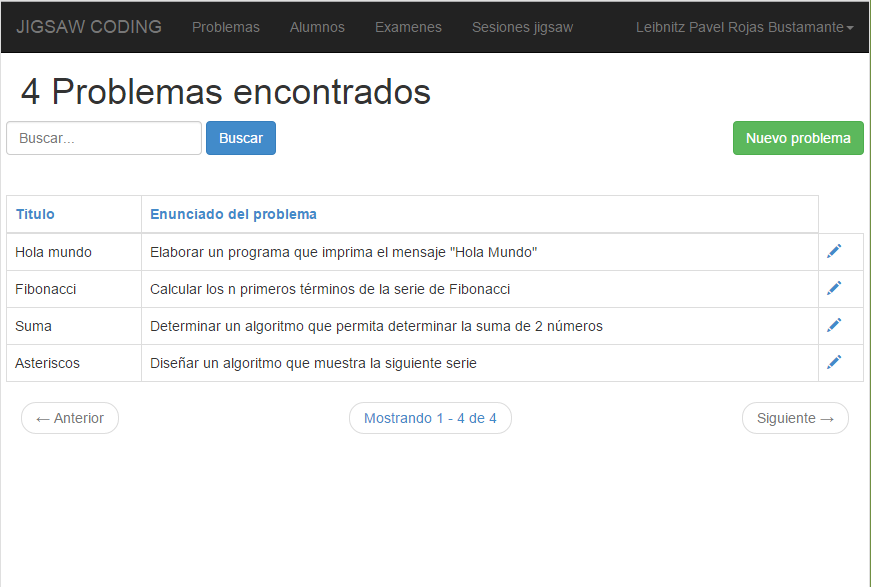
\includegraphics[scale=0.5]{figuras/usodelsistema/docente/problemas_inicio}
\end{figure}

\subsubsection{Crear nuevo problema}

Para crear un nuevo problema se debe acceder a menú Problemas y luego presionar el botón \textbf{Nuevo problema}. Ver figura \ref{fig:problemas_nuevo}. Luego, se debe ingresar el título y enunciado del problema y presionar el botón \textbf{Guardar}.

\begin{figure}[h!]
\centering
\caption[SJC Nuevo problema]{Sistema Jigsaw Coding - Nuevo problema}
\label{fig:problemas_nuevo}
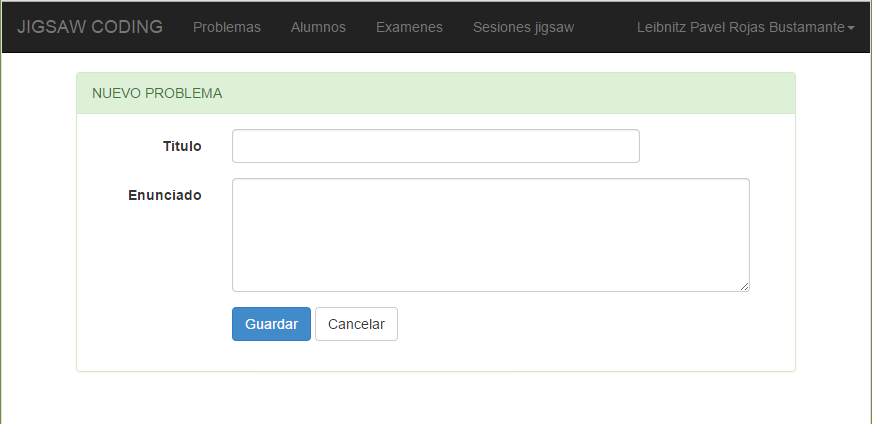
\includegraphics[scale=0.5]{figuras/usodelsistema/docente/problemas_nuevo}
\end{figure}

\subsubsection{Editar problema}
En la página principal del módulo Problemas se puede ver cada problema creado y para cada uno, existe un botón que permite editar dicho problema. Con esta opción se puede modificar el título o enunciado del problema y también se puede eliminar dicho problema del sistema. Ver figura \ref{fig:problemas_editar}.

\begin{figure}[h!]
\centering
\caption[SJC Editar problema]{Sistema Jigsaw Coding - Editar problema}
\label{fig:problemas_editar}
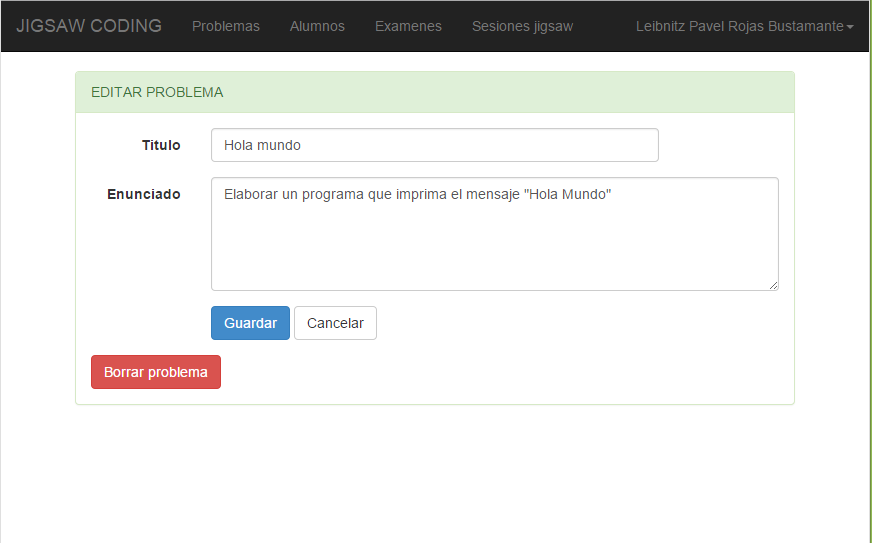
\includegraphics[scale=0.5]{figuras/usodelsistema/docente/problemas_editar}
\end{figure}

\subsection{Alumnos}
Al acceder al módulo alumnos, el usuario visualizará el listado de alumnos registrados hasta el momento y en dicho listado, se mostrará los apellidos, nombres y dni de cada alumno. Además se podrá filtrar dichos alumnos con opción Buscar.

\begin{figure}[h!]
	\centering
	\caption[SJC Alumnos]{Sistema Jigsaw Coding - Inicio del módulo Alumnos}
	\label{fig:alumnos_nuevo}
	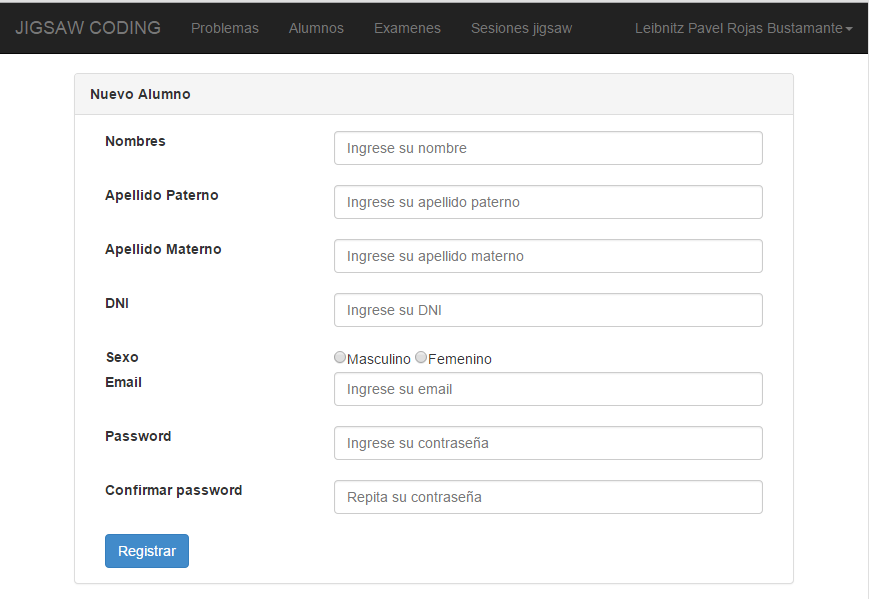
\includegraphics[scale=0.5]{figuras/usodelsistema/docente/alumnos_nuevo}
\end{figure}

\subsubsection{Registrar nuevo alumno}

Para registrar un nuevo alumno se debe acceder a menú Alumnos y luego presionar el botón \textbf{Nuevo Alumno}. Ver figura \ref{fig:alumnos_nuevo}. Luego, se debe completar los campos solicitados por el sistema y presionar el botón \textbf{Registrar}.

\begin{figure}[h!]
	\centering
	\caption[SJC Nuevo alumno]{Sistema Jigsaw Coding - Nuevo Alumno}
	\label{fig:alumnos_nuevo}
	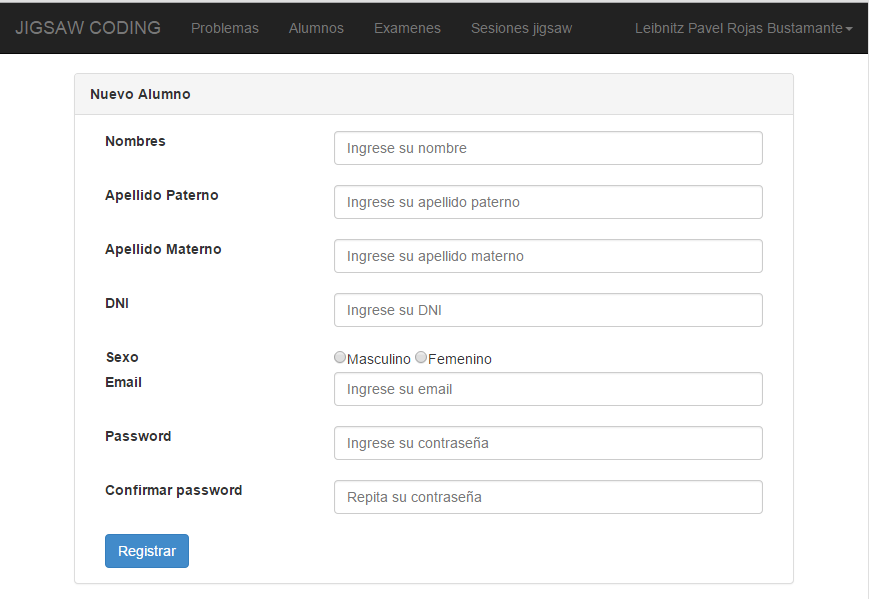
\includegraphics[scale=0.5]{figuras/usodelsistema/docente/alumnos_nuevo}
\end{figure}

\clearpage
\section{Definición de métricas de calidad para el Sistema Jigsaw Coding}





















































